\chapter{Implementacja}
Aplikacje testowe miały za zadanie sprawdzać dostępność najczęściej wykorzystywanych mechanizmów używanych do budowy aplikacji internetowych. Aby rozwiązywały one rzeczywisty problem, miały one pełnić rolę aplikacji do zarządzania inteligentnym budynkiem. Tematyka ta nawiązuje do mojej pracy inżynierskiej, której tematem był ,,System zarządzania inteligentnym domem z wykorzystaniem Raspberry Pi oraz technologii internetowych''.

W każdej z aplikacji zostały zaimplementowane następujące funkcjonalności:
\begin{itemize}
  \item rejestracja i logowanie użytkowników - system autentykacji,
  \item dodawanie i usuwanie sensorów,
  \item dodawanie i usuwanie danych zbieranych przez sensory,
  \item przetwarzanie danych w tle na przykładzie przetwarzania plików CSV z danymi użytkowników.
\end{itemize}

Każda z aplikacji obsługuje bazę danych o strukturze, która przedstawiona jest na rysunku \ref{fig:diagram_erd}.

\begin{figure}[h]
  \centering
  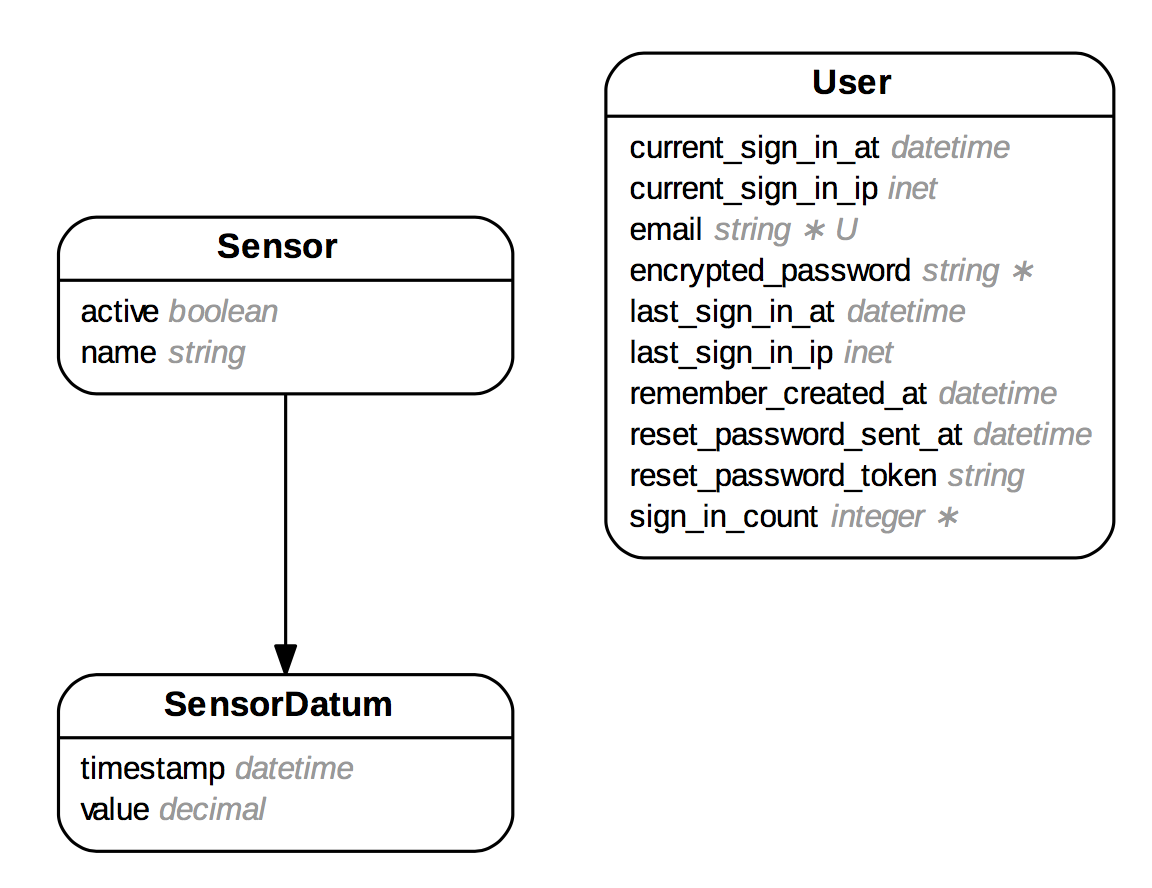
\includegraphics[width=\linewidth]{images/diagram_erd}
  \caption{Diagram ERD bazy danych.\\Źródło: opracowanie własne.}
  \label{fig:diagram_erd}
\end{figure}
\newpage
\section{Ruby on Rails}
Framework \emph{Ruby on Rails} domyślnie korzysta z architektury \emph{MVC}. Aby nie łamać zasady \emph{Convention over Configuration}, zdecydowano się stworzyć aplikację zgodną z ideą frameworka, czyli w tej właśnie architekturze.

\subsection{Modele}
Aplikacja posiada 3 modele: \emph{User}, \emph{TemperatureSensor} oraz \emph{TemperatureSensorDatum}. Dodatkowo, korzystając z mechanizmu \emph{STI} (ang. \emph{Single Table Inheritation}), istnieją dwa modele abstrakcyjne \emph{Sensor} oraz \emph{SensorDatum}, które są bazą dla różnych typów sensorów oraz danych zbierane przez owe sensory. Na listingach \ref{lst:rails_sensor} oraz \ref{lst:rails_temp_sensor} przedstawiony jest przykład implementacji \emph{STI}, czyli abstrakcyjny model sensora oraz dziedziczący po nim model \emph{TemperatureSensor}.
\newpage

\begin{lstlisting}[caption={Abstrakcyjny model sensora w Ruby on Rails.},label={lst:rails_sensor},language=Ruby]
class Sensor < ApplicationRecord
end
\end{lstlisting}

\begin{lstlisting}[caption={Model sensora temperatury w Ruby on Rails.},label={lst:rails_temp_sensor},language=Ruby]
class TemperatureSensor < Sensor
  has_many :temperature_sensor_data
end
\end{lstlisting}

Łatwo zauważyć, że abstrakcyjny model jest praktycznie pusty. Jedyną ważną informacją jest dziedziczenie po klasie \emph{ApplicationRecord}, po której musi dziedziczyć każdy model. Natomiast w klasie \emph{TemperatureSensor} zdefiniowana jest relacja jeden do wielu z danymi sensora.

\subsection{Kontrolery}
\emph{Ruby on Rails} posiada mechanizm, który pozwala na wygenerowanie szablonu kontrolera. Zawarte są w nim implementacje podstawowych operacji typu \emph{CRUD}, czyli \textbf{C}reate - \textbf{R}ead - \textbf{U}pdate - \textbf{D}elete. Jako, że z założenia nie ma możliwości edycji przychodzących danych, pominięta została sekcja \emph{Update}. Kontroler odpowiedzialny za dane z sensorów temperatury przedstawiony jest na listingu \ref{lst:rails_temp_controller}.

\begin{lstlisting}[caption={TemperatureSensorDataController w Ruby on Rails.},label={lst:rails_temp_controller},language=Ruby]
class TemperatureSensorDataController < ApplicationController
  before_action :set_temperature_sensor_datum, only: :destroy

  # GET /temperature_sensor_data
  def index
    @temperature_sensor_data = TemperatureSensorDatum.all
  end

  # GET /temperature_sensor_data/new
  def new
    @temperature_sensor_datum = TemperatureSensorDatum.new
  end

  # POST /temperature_sensor_data
  def create
    @temperature_sensor_datum = TemperatureSensorDatum.new(temperature_sensor_datum_params)
    respond_to do |format|
      if @temperature_sensor_datum.save
        format.html { redirect_to temperature_sensor_data_url, notice: 'Temperature sensor datum was successfully created.' }
      else
        format.html { render :new }
        format.json { render json: @temperature_sensor_datum.errors, status: :unprocessable_entity }
      end
    end
  end

  # DELETE /temperature_sensor_data/1
  def destroy
    @temperature_sensor_datum.destroy
    respond_to do |format|
      format.html { redirect_to temperature_sensor_data_url, notice: 'Temperature sensor datum was successfully destroyed.' }
      format.json { head :no_content }
    end
  end

  private
    # Use callbacks to share common setup or constraints between actions.
    def set_temperature_sensor_datum
      @temperature_sensor_datum = TemperatureSensorDatum.find(params[:id])
    end

    # Never trust parameters from the scary internet, only allow the white list through.
    def temperature_sensor_datum_params
      params.require(:temperature_sensor_datum).permit(:value, :timestamp, :sensor_id)
    end
end
\end{lstlisting}

\subsection{Widoki}
Każda z akcji w kontrolerze powinna mieć swój odpowiednik w warstwie widoków. Framework \emph{Ruby on Rails} dostarcza mechanizm \emph{partial'i}, który pozwala podział widoków na kilka plików w celu umożliwienia korzystania z jednego fragmentu w kilku miejscach. Przykład takiego rozwiązania można pokazać jako podstronę dodawania nowej próbki danych z sensora (listing \ref{lst:rails_sensor_data_view}), gdzie sam formularz jest reużywalnym fragmentem - \emph{partial'em} (listing \ref{lst:rails_sensor_form_partial}).

\begin{lstlisting}[caption={Widok, na którym można dodać nowe próbki dla sensora temperatury.},label={lst:rails_sensor_data_view},language=Ruby]
<h1>New Temperature Sensor Datum</h1>

<%= render 'form', temperature_sensor_datum: @temperature_sensor_datum %>

<%= link_to 'Back', temperature_sensor_data_path %>
\end{lstlisting}

\begin{lstlisting}[caption={Fragment, na którym jest formularz.},label={lst:rails_sensor_form_partial},language=Ruby]
<%= form_for(temperature_sensor_datum) do |f| %>
  <% if temperature_sensor_datum.errors.any? %>
    <div id="error_explanation"\>
      <h2><%= pluralize(temperature_sensor_datum.errors.count, "error") %> prohibited this temperature_sensor_datum from being saved:</h2>

      <ul>
      <% temperature_sensor_datum.errors.full_messages.each do |message| %>
        <li><%= message %></li>
      <% end %>
      </ul>
    </div>
  <% end %>

  <div class="field"\>
    <%= f.label :value %>
    <%= f.number_field :value, { step: 0.1 } %>
  </div\>

  <div class="field"\>
    <%= f.label :timestamp %>
    <%= f.datetime_local_field :timestamp %>
  </div>

  <div class="field"\>
    <%= f.label :sensor_id %>
    <%= f.collection_select(:sensor_id, TemperatureSensor.where(active: true), :id, :name) %>
  </div>

  <div class="actions"\>
    <%= f.submit %>
  </div>
<% end %>
\end{lstlisting}

\subsection{Przetwarzanie w tle - ActiveJob}
Framework \emph{Ruby on Rails} posiada wbudowany mechanizm, który jest abstrakcją umożliwiającą przetwarzanie danych w tle - \emph{ActiveJob}. Biblioteka ta posiada szereg adapterów do najbardziej popularnych mechanizmów zajmujących się owym przetwarzaniem. Dzięki temu możliwa jest ewentualna zmiana samego narzędzia, przy zachowaniu kodu. W aplikacji wykorzystane zostało narzędzie \emph{Sidekiq}.

Sam proces przetwarzania składa się z trzech części - widoku z formularzem, przy pomocy którego użytkowniok może wysłać plik csv na serwer, akcji w kontrolerze, która odbiera plik i przekazuje go do ostatniego etapu, czyli przetwarzania w tle. Na listingu \ref{lst:rails_active_job} przedstawiony został ostatni etap tego procesu.

\begin{lstlisting}[caption={},label={lst:rails_active_job},language=Ruby]
require "csv"
class UserImportJob < ApplicationJob
  queue_as :default

  def perform(file)
    CSV.foreach(file.path) do |row|
      User.create!(row.to_h)
    end
  end
end
\end{lstlisting}

\section{Phoenix}
\emph{Phoenix}, podobnie jak \emph{Ruby on Rails}, jest frameworkiem korzystającym z architektury \emph{Model-View-Controller}.

\subsection{Modele}
Jako, że \emph{Phoenix} nie posiada wbudowanego mechanizmu \emph{STI}, każdy model korzysta z osobnej tabeli w bazie danych. Oznacza to brak abstrakcyjnych modeli i ilość tabel w bazie danych równą ilości używanych modeli. Framework ten w modelu, poza relacjami z innymi modelami, przechowuje schemat danych w tabeli, z której korzysta dany model.

\begin{lstlisting}[caption={Model sensora temperatury we frameworku Phoenix.},label={lst:phoenix_temp_sensor_model}]
defmodule App.TemperatureSensor do
  use App.Web, :model

  schema "temperature_sensors" do
    field :name, :string
    field :active, :boolean, default: false

    timestamps()
  end

  def changeset(struct, params \\ %{}) do
    struct
    |> cast(params, [:name, :active])
    |> validate_required([:name, :active])
  end
end
\end{lstlisting}


\subsection{Kontrolery}
\emph{Phoenix} posiada mechanizm generowania \emph{scaffoldów}, które bardzo przyspieszają tworzenie aplikacji i generują sporą część kodu kontrolera, dzięki czemu można tworzyć proste aplikacje z minimalną znajomością języka programowania \emph{Elixir}. \emph{Scaffold} domyślnie generuje akcje kontrolera w konwencji \emph{CRUD}, lecz aby aplikacja była zgodna z wcześniejszymi założeniami, usunięta została część odpowiedzialna za edycję danych. Kontroler po tych zmianach przedstawiony jest na listingu \ref{lst:phoenix_controller}.

\begin{lstlisting}[caption={Kontroler danych z sensorów temperatur we frameworku Phoenix},label={lst:phoenix_controller}]
defmodule App.TemperatureSensorDatumController do
  use App.Web, :controller
  require IEx

  alias App.TemperatureSensorDatum
  alias App.TemperatureSensor

  def index(conn, _params) do
    temperature_sensor_data = Repo.all(TemperatureSensorDatum)
    render(conn, "index.html", temperature_sensor_data: temperature_sensor_data)
  end

  def new(conn, _params) do
    changeset = TemperatureSensorDatum.changeset(%TemperatureSensorDatum{})
    query = from(s in TemperatureSensor, select: {s.name, s.id})
    sensors = Repo.all(query)
    render(conn, "new.html", changeset: changeset, sensors: sensors)
  end

  def create(conn, %{"temperature_sensor_datum" => temperature_sensor_datum_params}) do
    temperature_sensor_datum_params =
      if temperature_sensor_datum_params["utc_timestamp"] do
        {:ok, timestamp} = DateTime.from_unix!(temperature_sensor_datum_params["utc_timestamp"])
        Map.put(temperature_sensor_datum_params, "utc_timestamp", timestamp)
      else
        temperature_sensor_datum_params
      end
    changeset = TemperatureSensorDatum.changeset(%TemperatureSensorDatum{}, temperature_sensor_datum_params)

    case Repo.insert(changeset) do
      {:ok, _temperature_sensor_datum} ->
        conn
        |> put_flash(:info, "Temperature sensor datum created successfully.")
        |> redirect(to: temperature_sensor_datum_path(conn, :index))
      {:error, changeset} ->
        query = from(s in TemperatureSensor, select: {s.name, s.id})
        sensors = Repo.all(query)
        render(conn, "new.html", changeset: changeset, sensors: sensors)
    end
  end

  def show(conn, %{"id" => id}) do
    temperature_sensor_datum = Repo.get!(TemperatureSensorDatum, id)
    render(conn, "show.html", temperature_sensor_datum: temperature_sensor_datum)
  end

  def delete(conn, %{"id" => id}) do
    temperature_sensor_datum = Repo.get!(TemperatureSensorDatum, id)

    # Here we use delete! (with a bang) because we expect
    # it to always work (and if it does not, it will raise).
    Repo.delete!(temperature_sensor_datum)

    conn
    |> put_flash(:info, "Temperature sensor datum deleted successfully.")
    |> redirect(to: temperature_sensor_datum_path(conn, :index))
  end
end
\end{lstlisting}

\subsection{Widoki}
W kwestii warstwy prezentacji widoczna jest inspiracja frameworkiem \emph{Ruby on Rails}. \emph{Phoenix} również posiada mechanizm fragmentów i działa on na takiej samej zasadzie, jak w oryginale.
\newpage

\begin{lstlisting}[caption={Widok, na którym można dodać dane dla sensora w  Phoenix'ie.},label={lst:phoenix_new_data_view},language=HTML]
<h2>New temperature sensor datum</h2>

<%= render "form.html", changeset: @changeset,
                        action: temperature_sensor_datum_path(@conn, :create),
                        sensors: @sensors %>

<%= link "Back", to: temperature_sensor_datum_path(@conn, :index) %>
\end{lstlisting}

\begin{lstlisting}[caption={Fragment, na którym jest formularz we frameworku Phoenix.},label={lst:phoenix_sensor_form_partial},language=HTML]
<%= form_for @changeset, @action, fn f -> %>
  <%= if @changeset.action do %>
    <div class="alert alert-danger"\>
      <p>Oops, something went wrong! Please check the errors below.</p>
    </div>
  <% end %>

  <div class="form-group"\>
    <%= label f, :value, class: "control-label" %>
    <%= number_input f, :value, step: "any", class: "form-control" %>
    <%= error_tag f, :value %>
  </div>

  <div class="form-group"\>
    <%= label f, :timestamp, class: "control-label" %>
    <%= datetime_select f,  :timestamp, class: "form-control" %>
    <%= error_tag f, :timestamp %>
  </div>

  <div class="form-group"\>
    <%= label f, :sensor_id, class: "control-label" %>
    <%= select(f, :sensor_id, @sensors) %>
  </div>

  <div class="form-group"\>
    <%= submit "Submit", class: "btn btn-primary" %>
  </div>
<% end %>
\end{lstlisting}

\subsection{Przetwarzanie danych w tle}
\emph{Phoenix} nie posiada wbudowanej biblioteki, która nakłada abstrakcję i unifikuje dostęp do mechanizmów odpowiedzialnych za przetwarzanie w tle. Nie oznacza to jednak, że realizacja przetwarzania danych w tle jest niemożliwa. Z pomocą przychodzi biblioteka \emph{Exq}. Sugeruje ona rozszerzenie istniejącej struktury o \emph{Workery}. Zaimplementowany \emph{worker} został przedstawiony na listingu \ref{lst:phoenix_worker}.

\begin{lstlisting}[caption={Worker umożliwiający import użytkowników z pliku csv we frameworku Phoenix.},label={lst:phoenix_worker}]
defmodule App.ImportUsersWorker do

  def perform(file) do
    File.stream!(file.path)
      |> CSV.decode(separator: ?;) |>
        Enum.each(fn row ->
          res = %{
            email: Enum.at(row, 0),
            password: Enum.at(row, 1),
            password_confirmation: Enum.at(row, 1)
          }
          User.changeset(%User{}, res)
          |> Repo.insert
        end)
  end
end
\end{lstlisting}

Aby dodać zadanie do kolejki, z poziomu kontrolera należy wywołać metodę przedstawioną na listingu \ref{lst:phoenix_worker_ctrl}

\begin{lstlisting}[caption={Dodanie zadania do kolejki przetwarzania w tle we frameworku Phoenix.},label={lst:phoenix_worker_ctrl}]
def import(conn, params) do
  {:ok, jid} = Exq.enqueue(Exq, "default", "ImportUsersWorker", [params["import"]["csv"]])
  text conn, "Task scheduled"
end
\end{lstlisting}

\section{Express}
\emph{Express} nie posiada domyślnie zdefiniowanej architektury, a więc również struktury projektu. Decyzja odnośnie architektury aplikacji leży w całości po stronie programisty. Aby zachować podobieństwo do pozostałych aplikacji, zdecydowano się na zastosowanie modelu \emph{Model-View-Controller}.

\subsection{Modele}
Korzystanie z modeli możliwe jest dzięki zastosowaniu biblioteki \emph{Sequelize.js}. W modelach zawarte są informacje na temat pól danego modelu i ich typów, a więc jego schemat. Dodatkowo, model zawiera informacje na temat relacji z innymi modelami.

\begin{lstlisting}[caption={Model sensora temperatury w Express'ie.},label={lst:express_temp_sensor_model}]
var Sequelize = require('sequelize')

var TemperatureSensor = connection.define('temperature_sensors',
                                        TemperatureSensorMeta.attributes,
                                        TemperatureSensorMeta.options)

TemperatureSensor.hasMany(TemperatureSensorDatum);

var attributes = {
  name: {
    type: Sequelize.STRING,
  },
  active: {
    type: Sequelize.BOOLEAN,
  }
}

var options = {
  freezeTableName: true
}

module.exports.attributes = attributes
module.exports.options = options
\end{lstlisting}

\subsection{Kontrolery}
W przeciwieństwie do \emph{Ruby on Rails} i \emph{Phoenix'a}, \emph{Express} nie posiada mechanizmu generowania \emph{scaffold'ów}. W efekcie wszystkie metody należy stworzyć samodzielnie, co ma wpływ na szybkość powstawania aplikacji, w której większośc akcji jest standardowych, czyli spełniających założenia \emph{CRUD}. Na listingu \ref{lst:express_temp_data_controller} przedstawiony jest kontroller we frameworku \emph{Express}.

\begin{lstlisting}[caption={Kontroler danych z sensora temperatury we frameworku Express.},label={lst:express_temp_data_controller}]
var Model = require('../model/models.js')

module.exports.index = function(req, res) {
  Model.TemperatureSensorDatum.findAll().then(data => {
    res.send(data)
  })
}

module.exports.create = function(req, res) {
  var value = req.body.temperature_sensor_datum.value
  var sensorId = req.body.temperature_sensor_datum.sensor_id

  var newTemperatureSensorDatum = {
    value: parseFloat(value),
    temperatureSensorId: sensorId
  }

  Model.TemperatureSensorDatum.create(newTemperatureSensorDatum).then(function() {
    res.redirect('/')
  }).catch(function(error) {
    res.send('error')
    req.flash('error', "Something went wrong...")
  })
}
\end{lstlisting}

\subsection{Widoki}
W implementacji warstwy widoków został wykorzystany silnik \emph{Handlebards}. Jest to popularne rozwiązanie, spotykane w innych frameworkach webowych zorientowanych na warstwę prezentacji. Przykładowym frameworkiem, który domyślnie korzysta z tego mechanizmu jest \emph{Ember.js}. System ten oparty jest o mechanizm \emph{layout'ów}, w których osadzane są konkretne podstrony. Dzięki temu możliwe jest zachowanie spójnego wyglądu na każdej z podstron. Na listingach \ref{lst:express_layout} oraz \ref{lst:express_view} przedstawiony jest layout strony oraz zawartość podstrony do rejestracji użytkownika.

\begin{lstlisting}[caption={Layout używany w aplikacji napisanej przy pomocy Express'a.},label={lst:express_layout},language=HTML]
<!DOCTYPE html>
<html>
<head>
  <meta charset="utf-8"\>
  <title>Example App</title>
  <!-- Bootstrap -->
  <link rel="stylesheet" href="https://maxcdn.bootstrapcdn.com/bootstrap/3.3.5/css/bootstrap.min.css"\>
  <link rel="stylesheet" href="https://maxcdn.bootstrapcdn.com/bootstrap/3.3.5/css/bootstrap-theme.min.css"\>

  <link rel="stylesheet" href="/styles/app.css"\>

  {{{_sections.head}}}
</head>
<body>
    {{{body}}}

    <!-- Bootstrap -->
    <script src="https://maxcdn.bootstrapcdn.com/bootstrap/3.3.5/js/bootstrap.min.js"\></script>
    <!-- IE10 viewport hack for Surface/desktop Windows 8 bug -->
    <script src="../../assets/js/ie10-viewport-bug-workaround.js"\></script>
</body>
</html>
\end{lstlisting}

\newpage
\begin{lstlisting}[caption={Podstrona rejestracji użytkownika w Express'ie.},label={lst:express_view},language=HTML]
{{#section 'head'}}
    <link rel="stylesheet" href="/styles/auth.css"\>
{{/section}}

<div class="container"\>
  <form method="POST" action="/users/sign_up" class="form-signin"\>
    <h2 class="form-signin-heading"\>Create an account</h2>

    {{#if errorMessage}}
      <div class="alert alert-danger"\>
        {{errorMessage}}
      </div>
    {{/if}}

    <label for="inputEmail" class="sr-only"\>Email</label>
    <input type="text" id="inputEmail" name="email" class="form-control" placeholder="Email" required autofocus>
    <label for="inputPassword" class="sr-only"\>Password</label>
    <input type="password" id="inputPassword" name="password" class="form-control" placeholder="Password" required>
    <label for="inputPassword" class="sr-only"\>Repeat Password</label>
    <input type="password" id="inputPassword2" name="password2" class="form-control" placeholder="Repeat Password" required>
    <button class="btn btn-lg btn-primary btn-block" type="submit"\>Sign up</button>
  </form>
</div>
\end{lstlisting}
